\section{TimeSets Visualization}

\subsection{Events}
In TimeSets, an event is visualized as a line of text, showing its \emph{label}. The visual indicator of event time is a circle (for a time-point event), or a horizontal bar (for an interval event). The \textit{time circle} is shown to the left of the label, while the \textit{time bar} is shown above the label. The time bar is semi-transparent for overlapping interval events, so the intersection part is visually different. To accommodate a large number of events, labels have three possible levels of detail: 
\begin{itemize}
	\item Complete: the entire event label is shown.
	\item Trimmed: only the first few words are shown, followed by three dots at the end.
	\item Aggregated: a few events are combined into a new one with its label indicating the number of events, such as ``2 events''.
\end{itemize}	
The text border of an aggregated event is colored to make it visually different from non-aggregated events. Its time bar begins at the starting time of the earliest event, and ends at the finishing time of the latest event within the aggregate. Figure~\ref{fig:event-representation} shows a complete time-point, a trimmed time-point, an interval, an aggregate of two events, and two overlapping interval events.

\begin{figure}[ht]
\centering
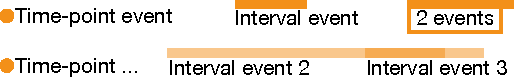
\includegraphics[width=.8\columnwidth]{figure2}
\caption{Visual representations of complete and trimmed time-point events, interval, aggregated, and overlapping events.}
\label{fig:event-representation}
\end{figure}

\subsection{Sets}
\subsubsection{Design Overview}
As discussed in the related work, Gestalt principles of grouping are commonly used to show set relationships among events, most effectively uniform connectedness and proximity. Therefore, we also apply these two principles in our design. Proximity is achieved by moving same-set events close together, and coloring the set background makes the events visually connected.

Because the horizontal position of each event is decided by its timestamp, spatial grouping is achieved through vertical positioning. The sets are stacked vertically, and each set is further divided into a maximum of three horizontal \emph{layers}: a top and a bottom layer for events shared with the set above and below respectively (if they exist), and a middle layer for other events in the set. There are maximal $2n-1$ layers in total for $n$ sets of events. Figure~\ref{fig:layering} shows the layering for three sets. 

\begin{figure}[ht]
\centering
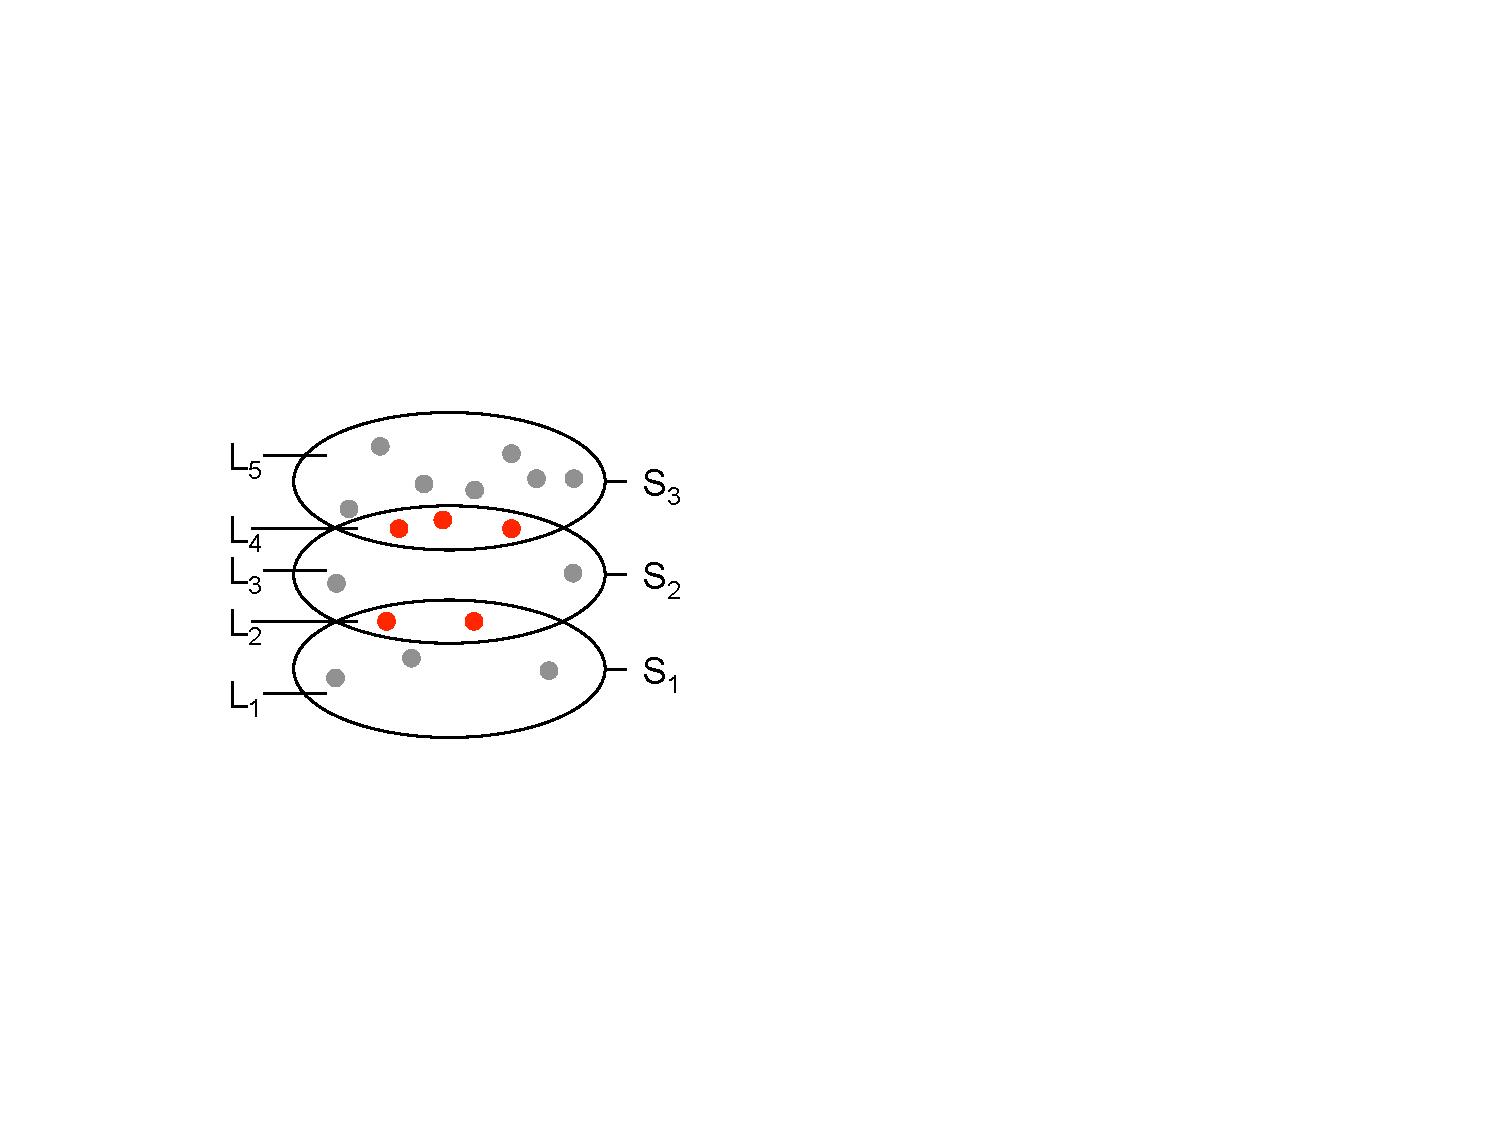
\includegraphics[width=.5\columnwidth]{figure3}
\caption{Layering for three sets $S_1$, $S_2$, and $S_3$. $L_2$ consists of events shared by $S_1$ and $S_2$, and $L_4$ consists of events shared by $S_2$ and $S_3$. Those shared events are red circles.}
\label{fig:layering}
\end{figure}

\begin{figure}[ht]
	\centering
	\subcaptionbox{Visual links connect shared events from one set to another set.}[.46\columnwidth]
		{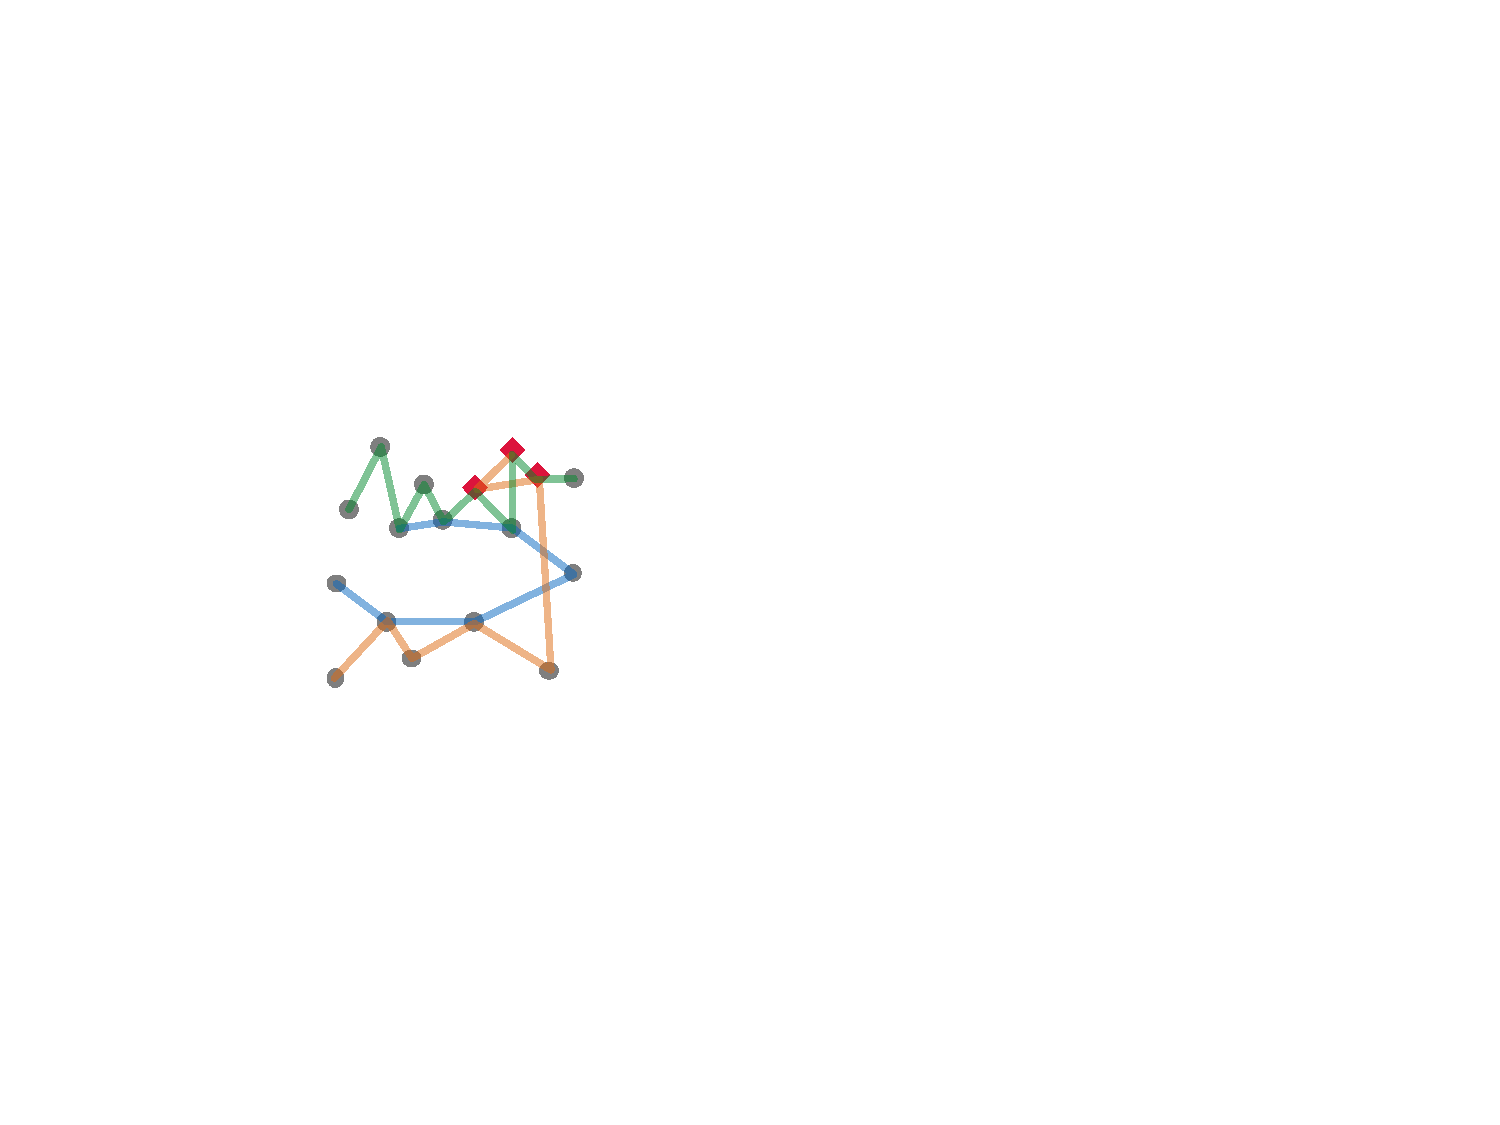
\includegraphics[width=.35\columnwidth]{figure4a}}\label{fig:layering-1}
	\hfill	
	\subcaptionbox{Shared events are duplicated in both sets.}[.46\columnwidth]
		{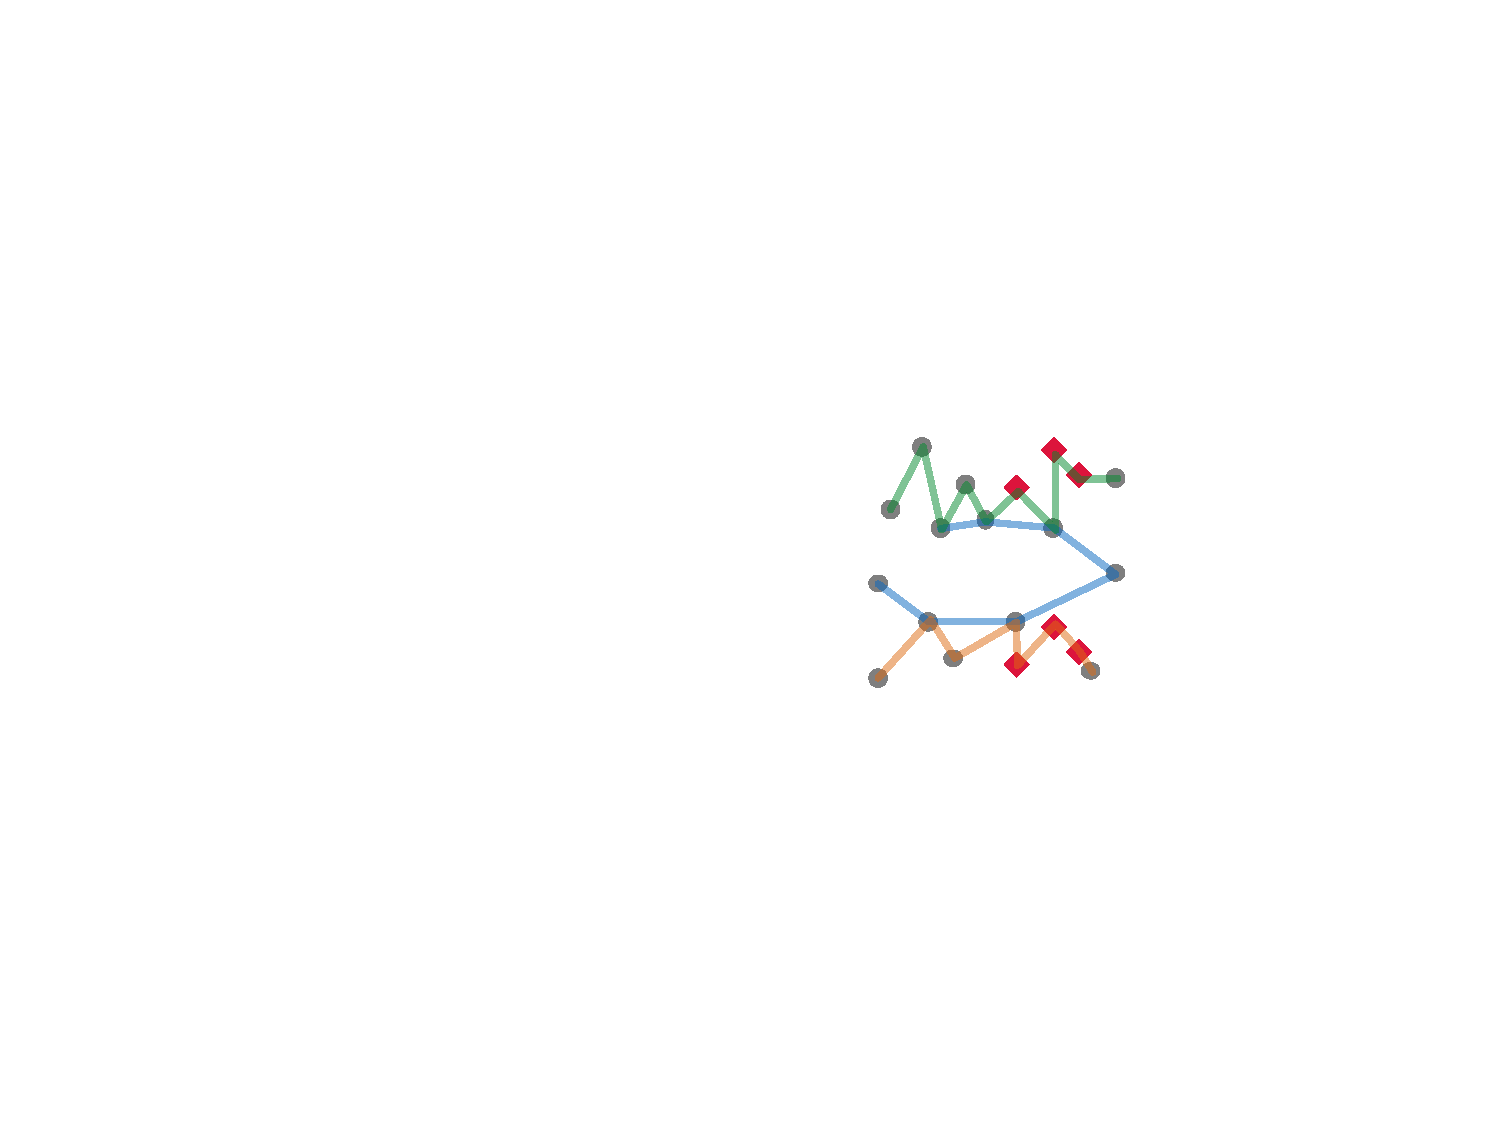
\includegraphics[width=.35\columnwidth]{figure4b}}\label{fig:layering-2}
	\caption{Visualizing shared events (red squares) between two non-neighboring sets.}
	\label{fig:layering-compare}
\end{figure}

Shared events between two non-neighboring sets can reside in one set and connect to the other set using visual links such as curves~\cite{Alper2011} or areas~\cite{Meulemans2013}. Figure~\ref{fig:layering-1} shows a possible method of connecting the shared events (red squares) using edges and linking them to the yellow set to indicate that they also belong to that set. The alternative approach is to duplicate them in both sets. In Figure~\ref{fig:layering-2}, red squares are duplicated in both the blue and yellow sets. Duplication consumes more display space and could make viewers confuse when seeing same events multiple times. However, duplication allows all events of a same set being placed close together, which provides a compact visualization and easy comparison. Also, the study by Henry Riche and Dwyer~\cite{Riche2010} shows that complex set intersection shapes reduce readability compared to item duplication. Aiming for a clear visualization, we decided to duplicate events that belong to non-neighboring sets. Confused duplication and scalability will be addressed later using interaction and layout algorithm respectively.

In subsequent sections, we discuss the detail of the set visualization algorithm, which consists of two main steps: the generation of set shapes, and then their coloring.

\subsubsection{Shape Generation}
\label{sub:shapesgeneration}
This algorithm takes as input a list of bounding-boxes of the set's events, and generates a closed-curve containing all these rectangles. The sizes and positions of the bounding boxes are decided by the layout algorithm described in the next section. A rectilinear shape can be generated using the scan-line algorithm~\cite{Foley1997}, as shown in Figure~\ref{fig:shape1}. The number of bends along the line is often used to assess the aesthetics and legibility of visualizations~\cite{Tanahashi2012}. Even though the generated shape provides the minimal \textit{data-ink} ratio~\cite{Tufte1986}, a large number of line bends may reduce its legibility. 

\begin{figure}[ht]
	\centering
	\subcaptionbox{The rectilinear shape, generated by a scan-line algorithm.} 
		{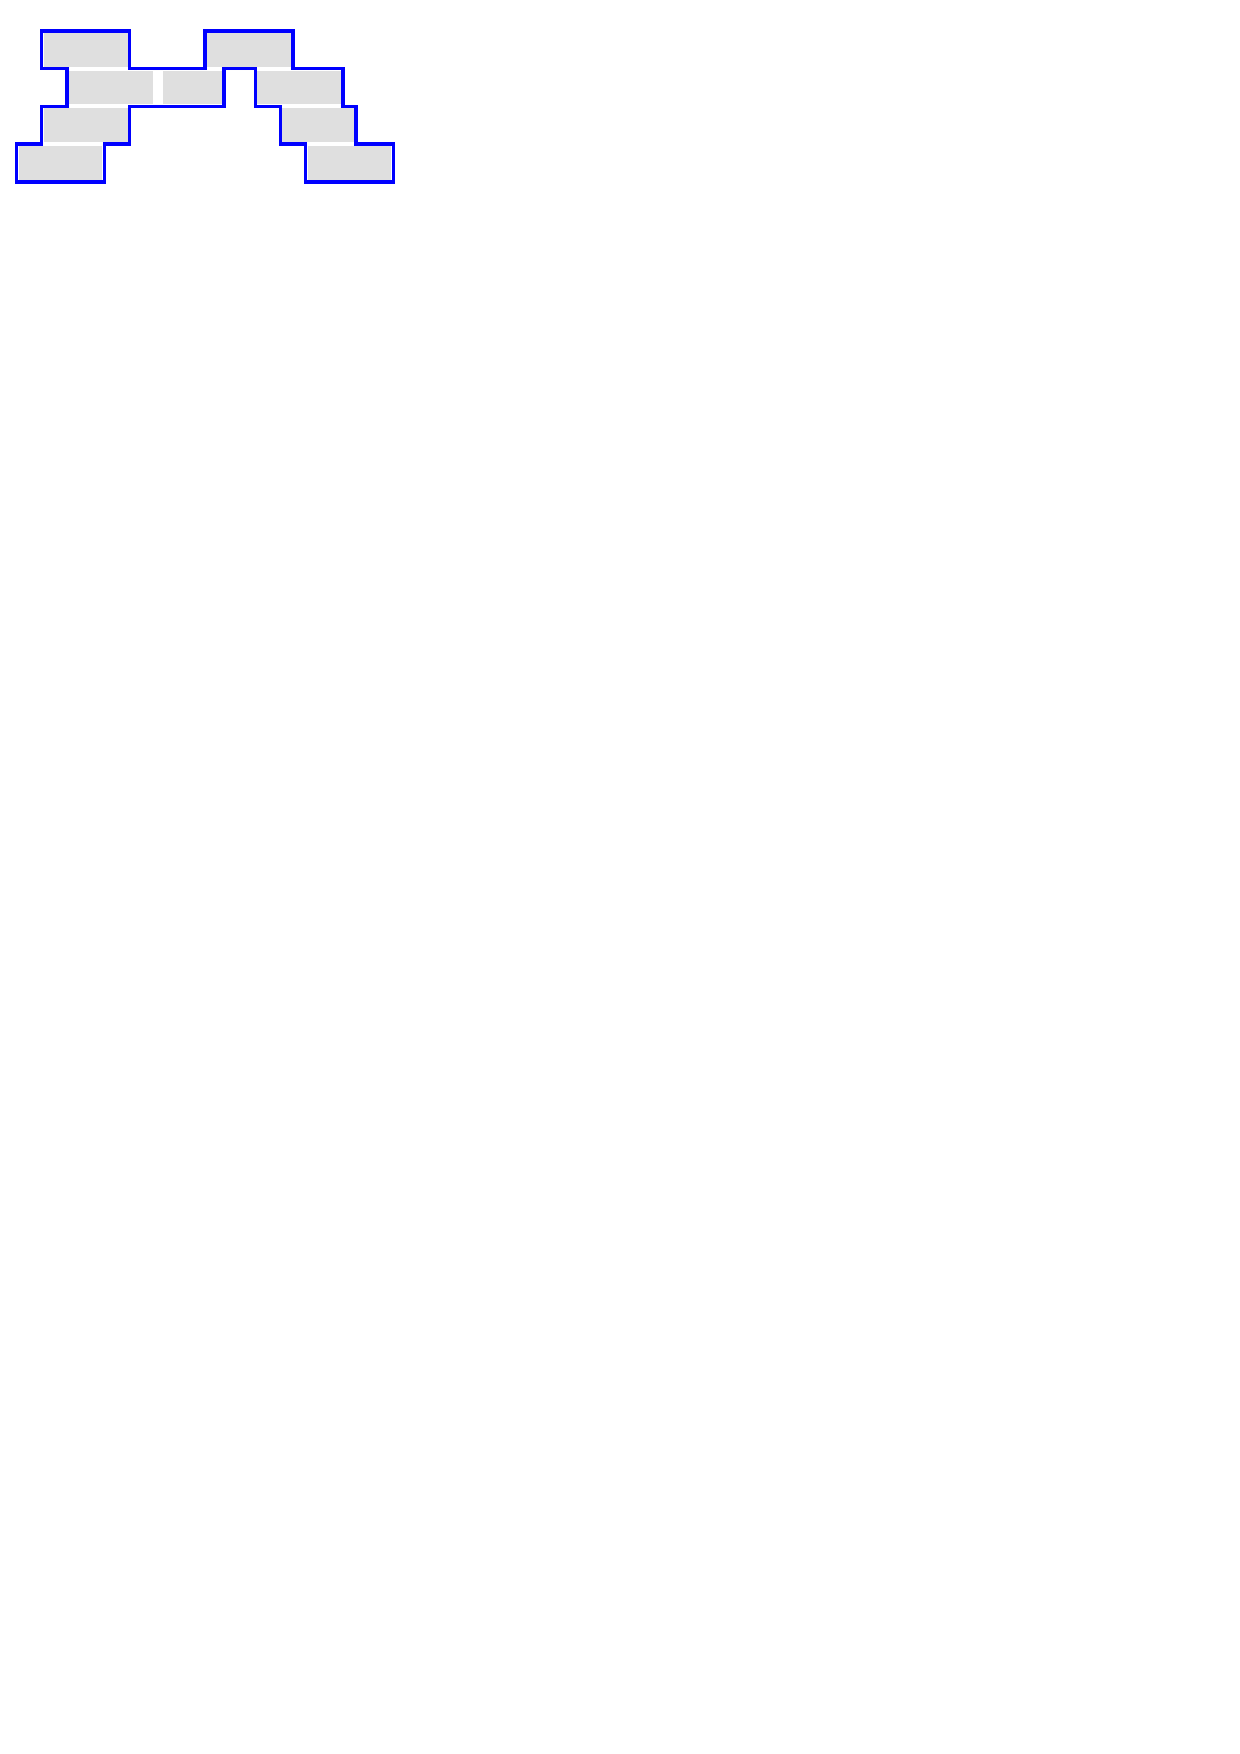
\includegraphics[width=.47\columnwidth]{figure5a}}\label{fig:shape1}
	\hfill
	\subcaptionbox{The simplified shape by flattening and removing jags (red eclipse).}
		{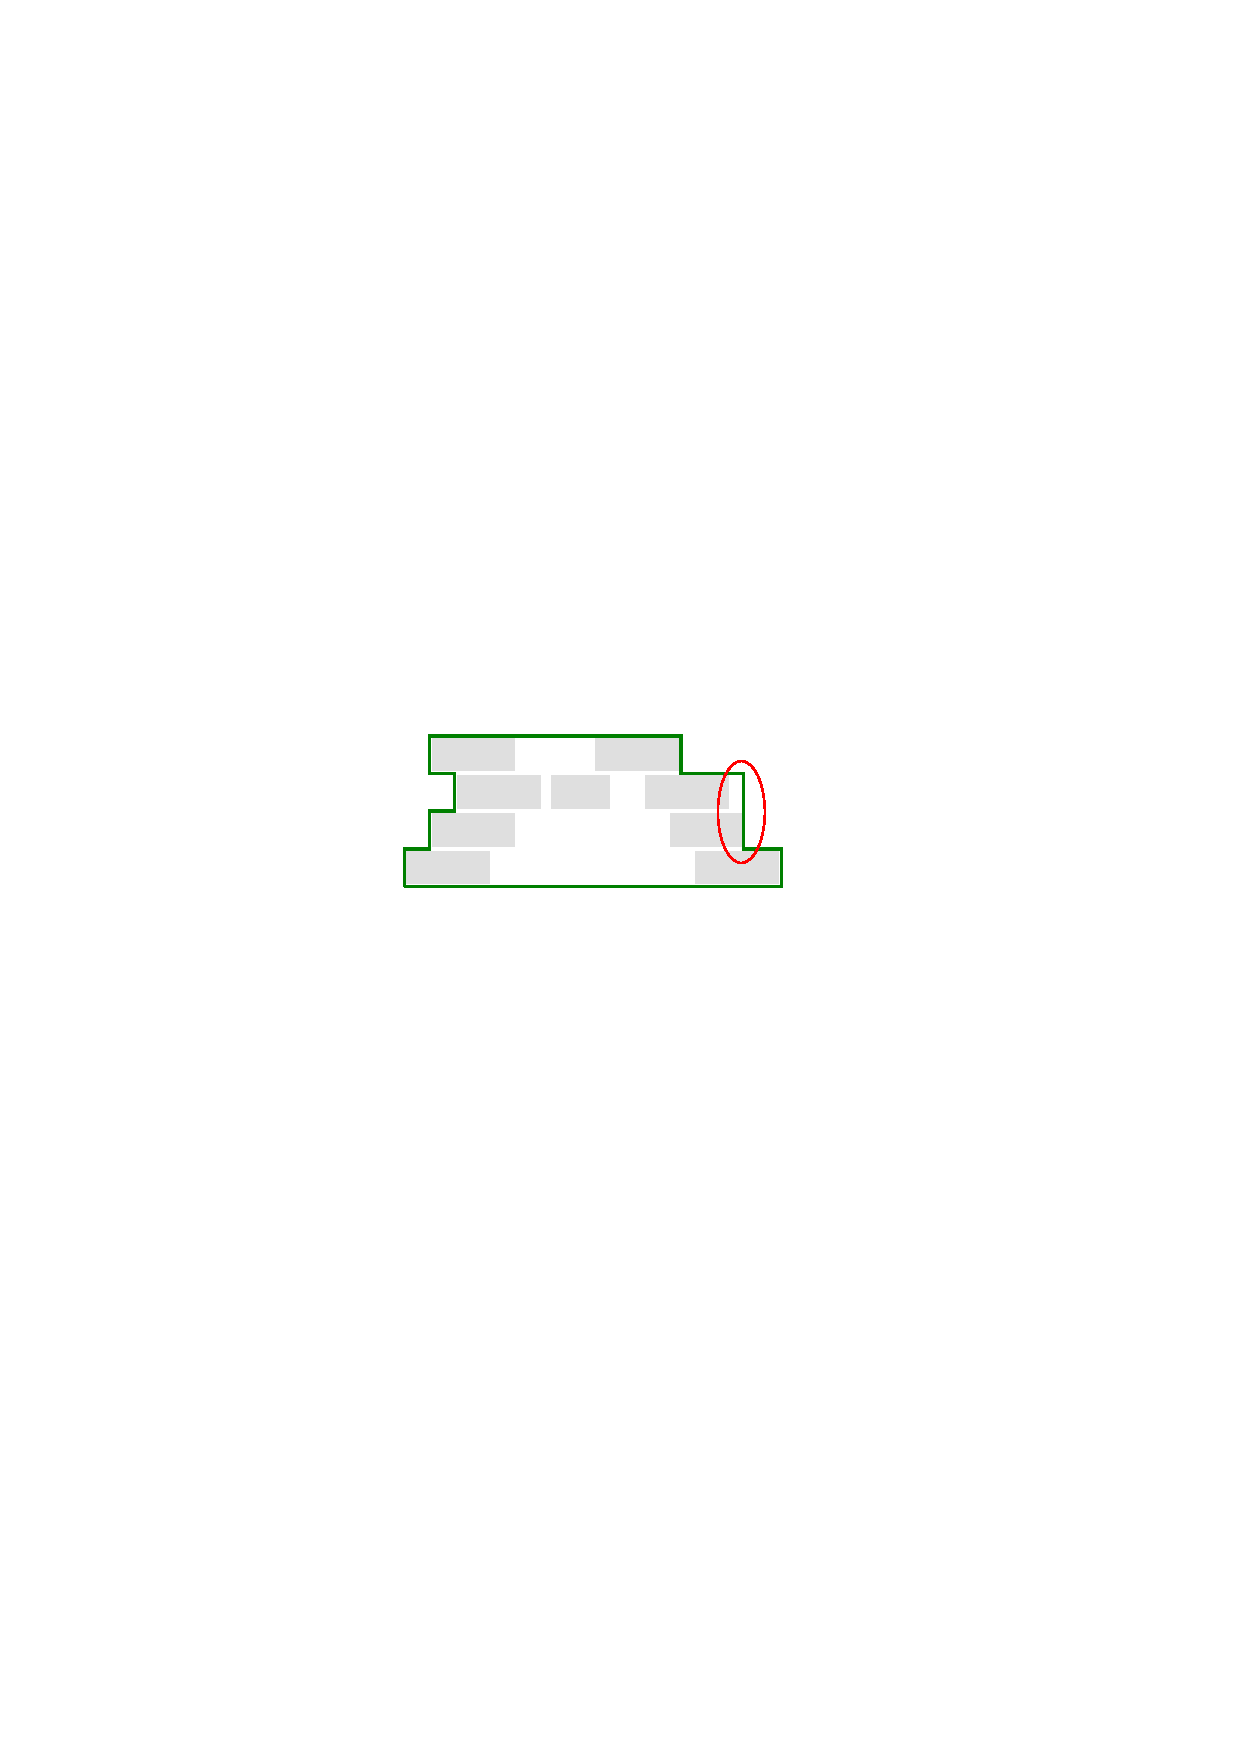
\includegraphics[width=.47\columnwidth]{figure5b}}\label{fig:shape2}
	\caption{Rectilinear shape generation.}
	\label{fig:shape}
\end{figure}

To reduce the number of line bends, the top and the bottom sides of the set outline are flattened. The left and right sides  are kept unchanged because they indicate the event timespan. On either side, the path can be ``jagged'' if two events start or end close to each other. Those close vertical segments are combined to reduce line bends if their horizontal gap is smaller than a threshold. This trades off time accuracy for outline smoothness and can be controlled by the user. Figure~\ref{fig:shape2} shows the result of this simplification. 

To reduce the degree of line bends, the algorithm converts vertical segments to diagonal ones wherever possible, such as  $e_2$ and $e_3$ in Figure~\ref{fig:generation1}. Smoother lines are easier to follow~\cite{Kim2010}, thus the algorithm further converts diagonal segments to B\'{e}zier curves and replaces right corners with quadrant arcs as in Figure~\ref{fig:generation2}.

\begin{figure}[ht]
	\centering
	\subcaptionbox{Vertical segments $e_2$ and $e_3$ are converted to diagonal ones (dashed lines).}
		{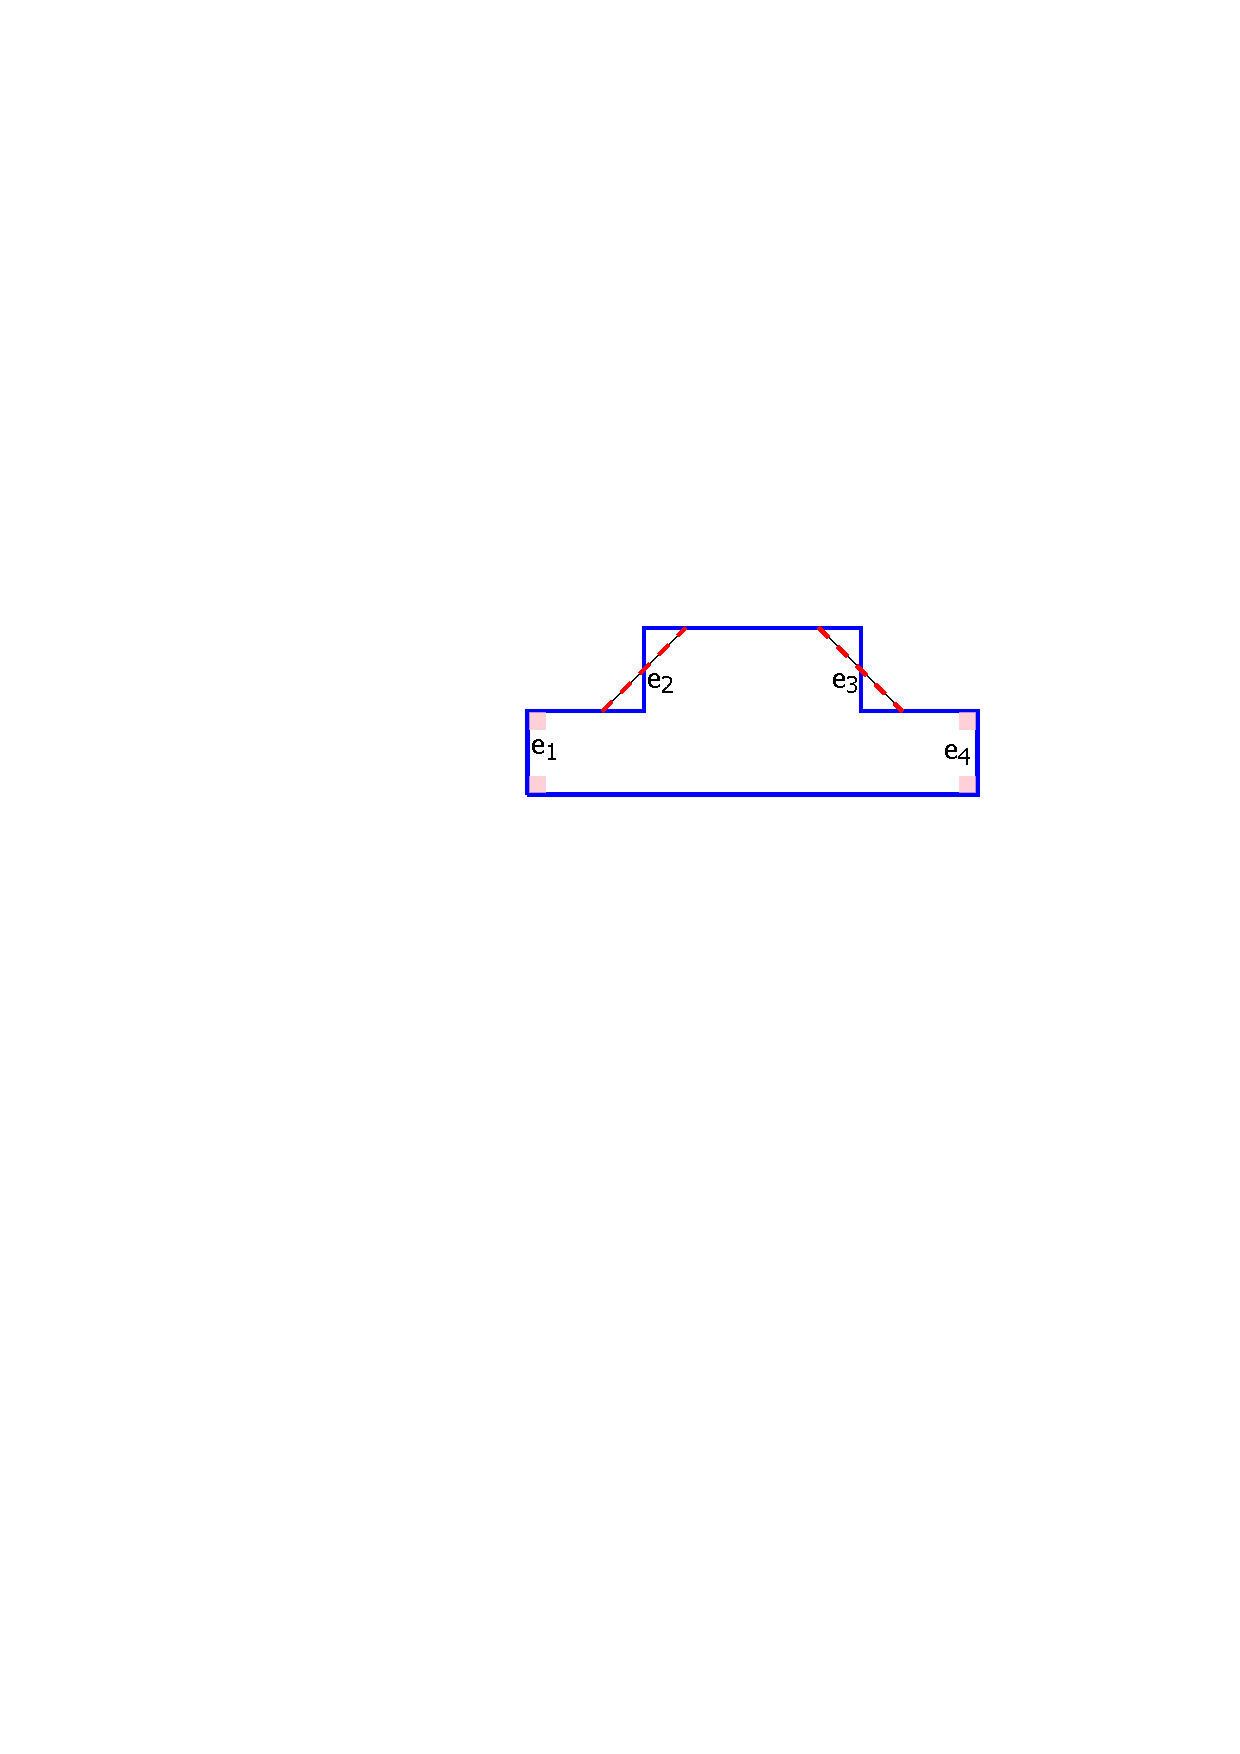
\includegraphics[width=.47\columnwidth]{figure6a}}\label{fig:generation1}
	\hfill
	\subcaptionbox{Right corners are replaced by quadrants. $e_2$ and $e_3$ are smoothened by B\'{e}zier curves.}
		{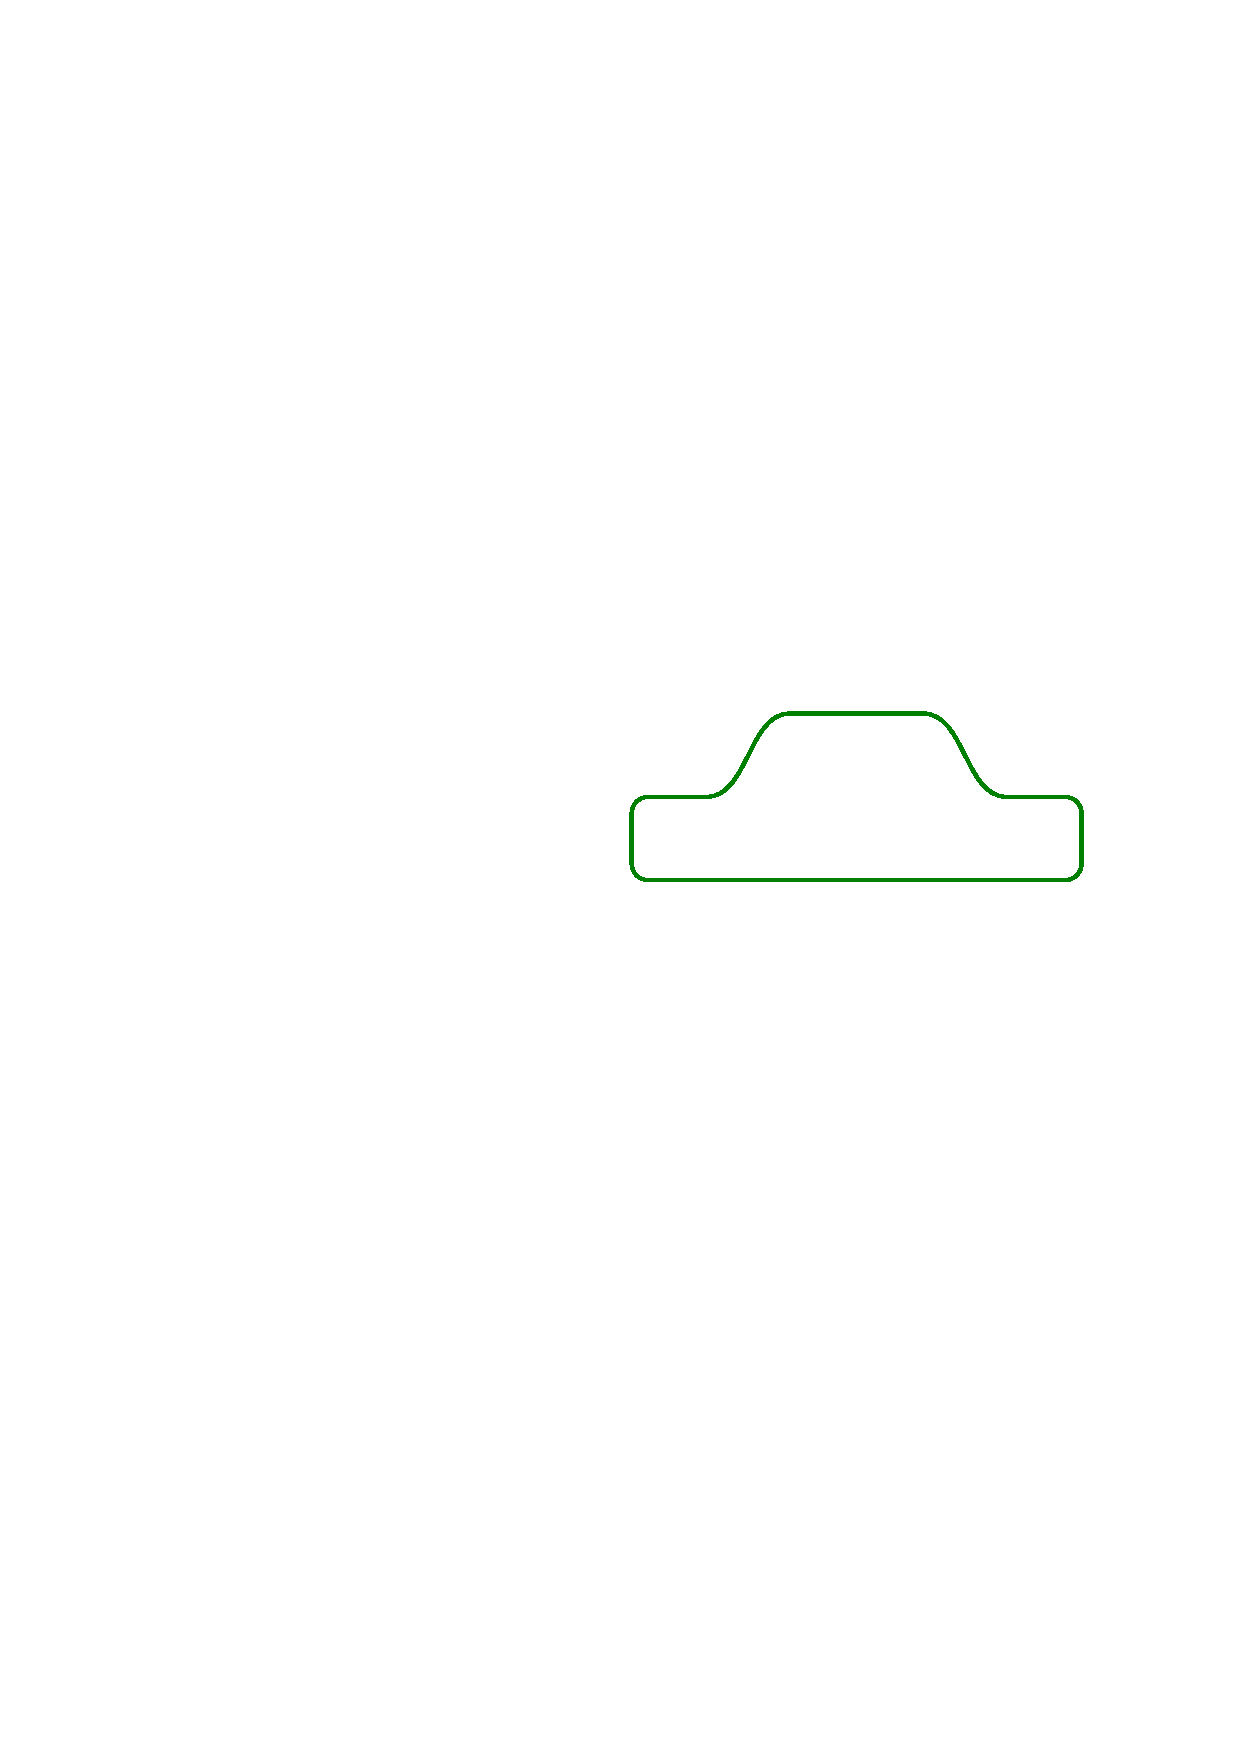
\includegraphics[width=.47\columnwidth]{figure6b}}\label{fig:generation2}
	\caption{Shape smoothening by reducing the degree of line bends.}
	\label{fig:generation}
\end{figure}

\subsubsection{Coloring}
Each set is filled with a color selected from Qualitative Set 2 of ColorBrewer~\cite{Harrower2003} to make them easily distinguishable. Two color filling options are considered: only the time circle or the entire event label. Our design follows uniform connectedness principle requiring visual connection among same-set events. When they are visually connected and only their time circles are filled, additional edges may reduce the readability. KelpFusion~\cite{Meulemans2013} follows this approach using lines and areas to connect time circles reducing its readability as in Figure~\ref{fig:evaluation2}. In the second option, filling the entire label may produce a false impression about the event's time range. We choose this option and lessen the effect by coloring the gap between events as in Figure~\ref{fig:evaluation1}. It also helps increase the sense of grouping compared to filling only the time circles.

The standard coloring method for set intersections is color blending as commonly used for Venn diagrams~\cite{Ware2013}. Color for each set is half-transparent, and alpha blending is applied to produce the new color for the intersection. However, the result may be irrelevant to the two inputs and confused as the color for a new set. For instance, in Figure~\ref{fig:layering}, the yellow color of layer $L_2$ is not naturally considered as the common between light yellow of set $S_1$ and light green of set $S_2$.

To address this issue, we fill the intersection with a linear color gradient changing between the two set colors as in Figure~\ref{fig:gradient1}. While the gradient provides a smooth transition, it becomes difficult to recognize the two ends of the intersection. For example, it is not clear from Figure~\ref{fig:gradient1} that the background of the event \textit{Rove's 4th grand jury appearance} (2\textsuperscript{nd} row top down) is pure yellow or it has a mix of green as well. To solve this problem, multiple color transitions are used instead of a single transition. For instance, in Figure~\ref{fig:gradient2}, the color transitions between green and yellow are repeated multiple times so that both colors are clearly shown in every row of the intersection, and there is no significant difference in color perception among these rows.

\begin{figure}[ht]
	\centering
	\subcaptionbox{Intersection shown as a single color gradient.}
		{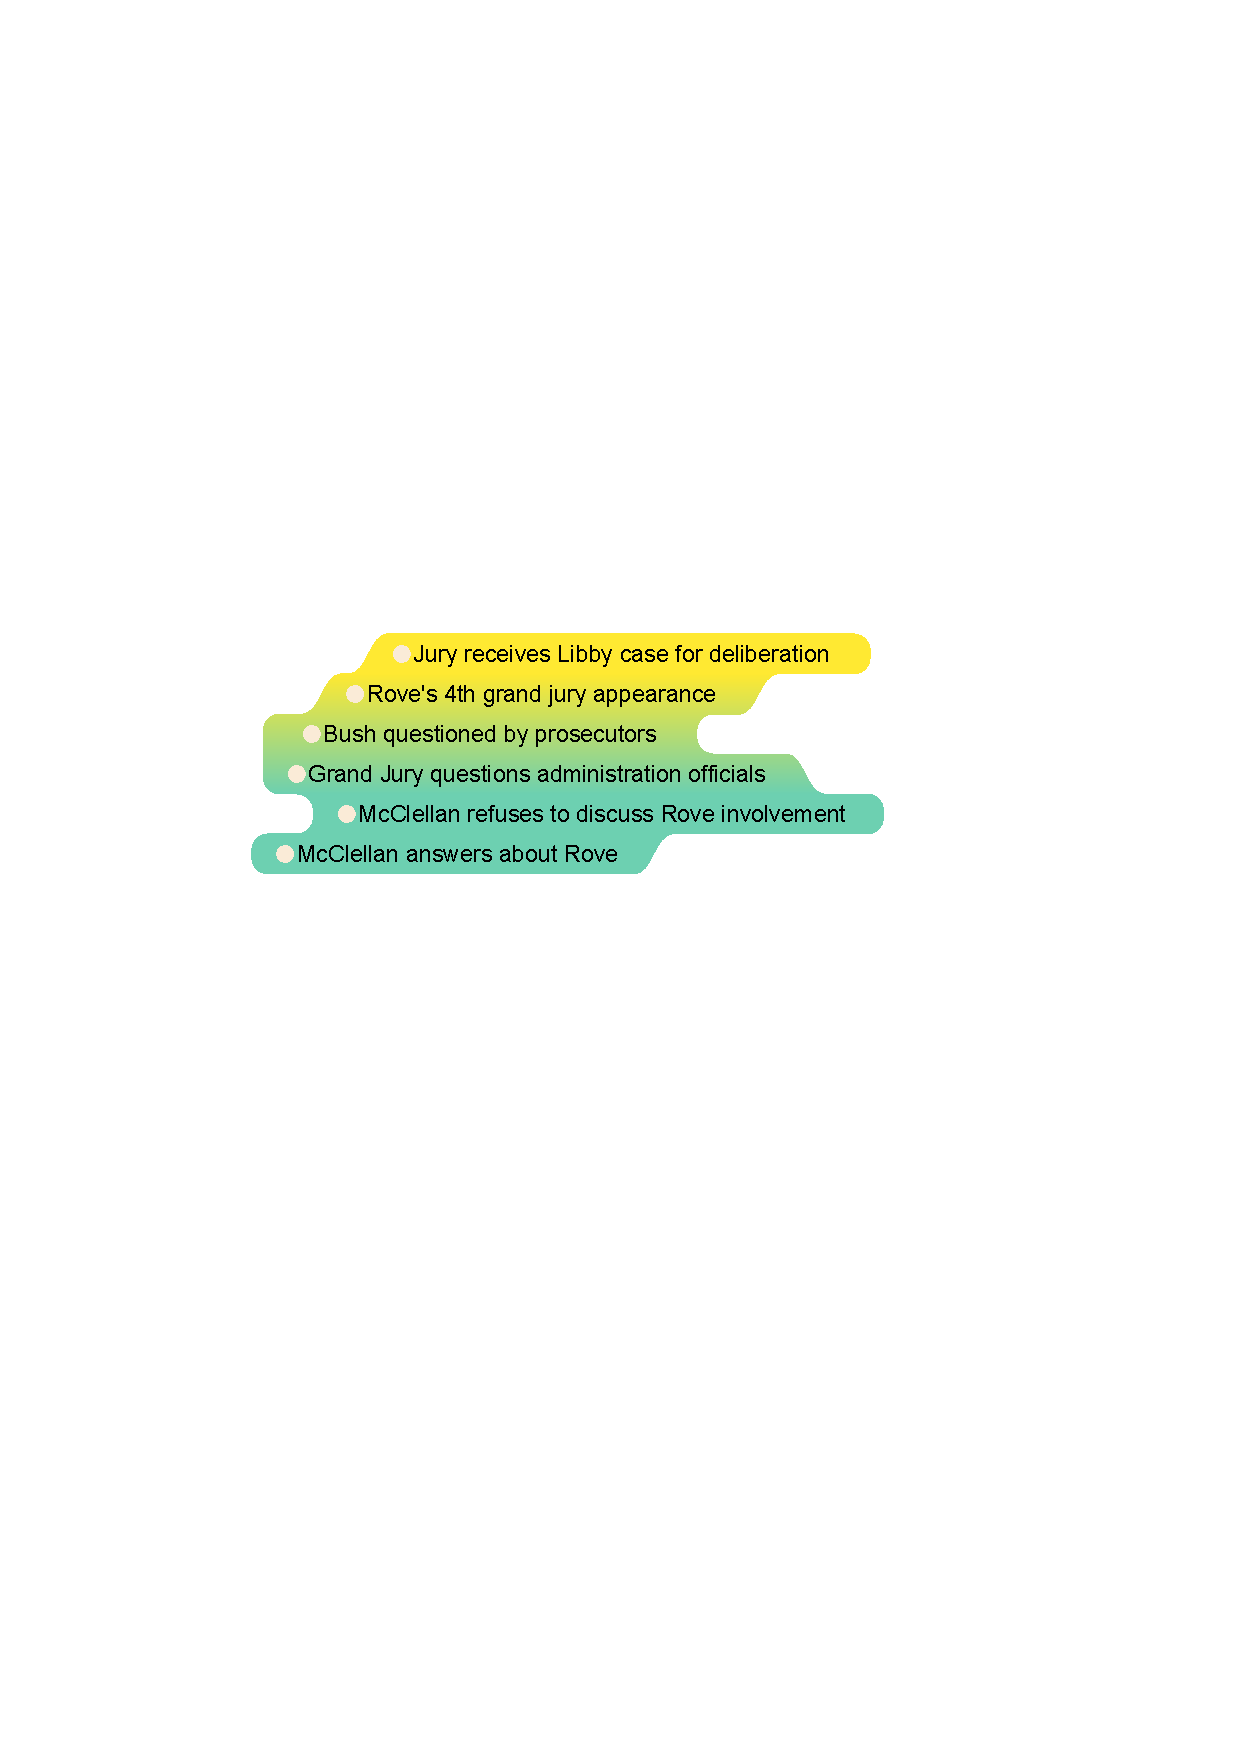
\includegraphics[width=0.48\columnwidth]{figure7a}}\label{fig:gradient1}
	\hfill
	\subcaptionbox{Intersection shown as multiple color gradients.}
		{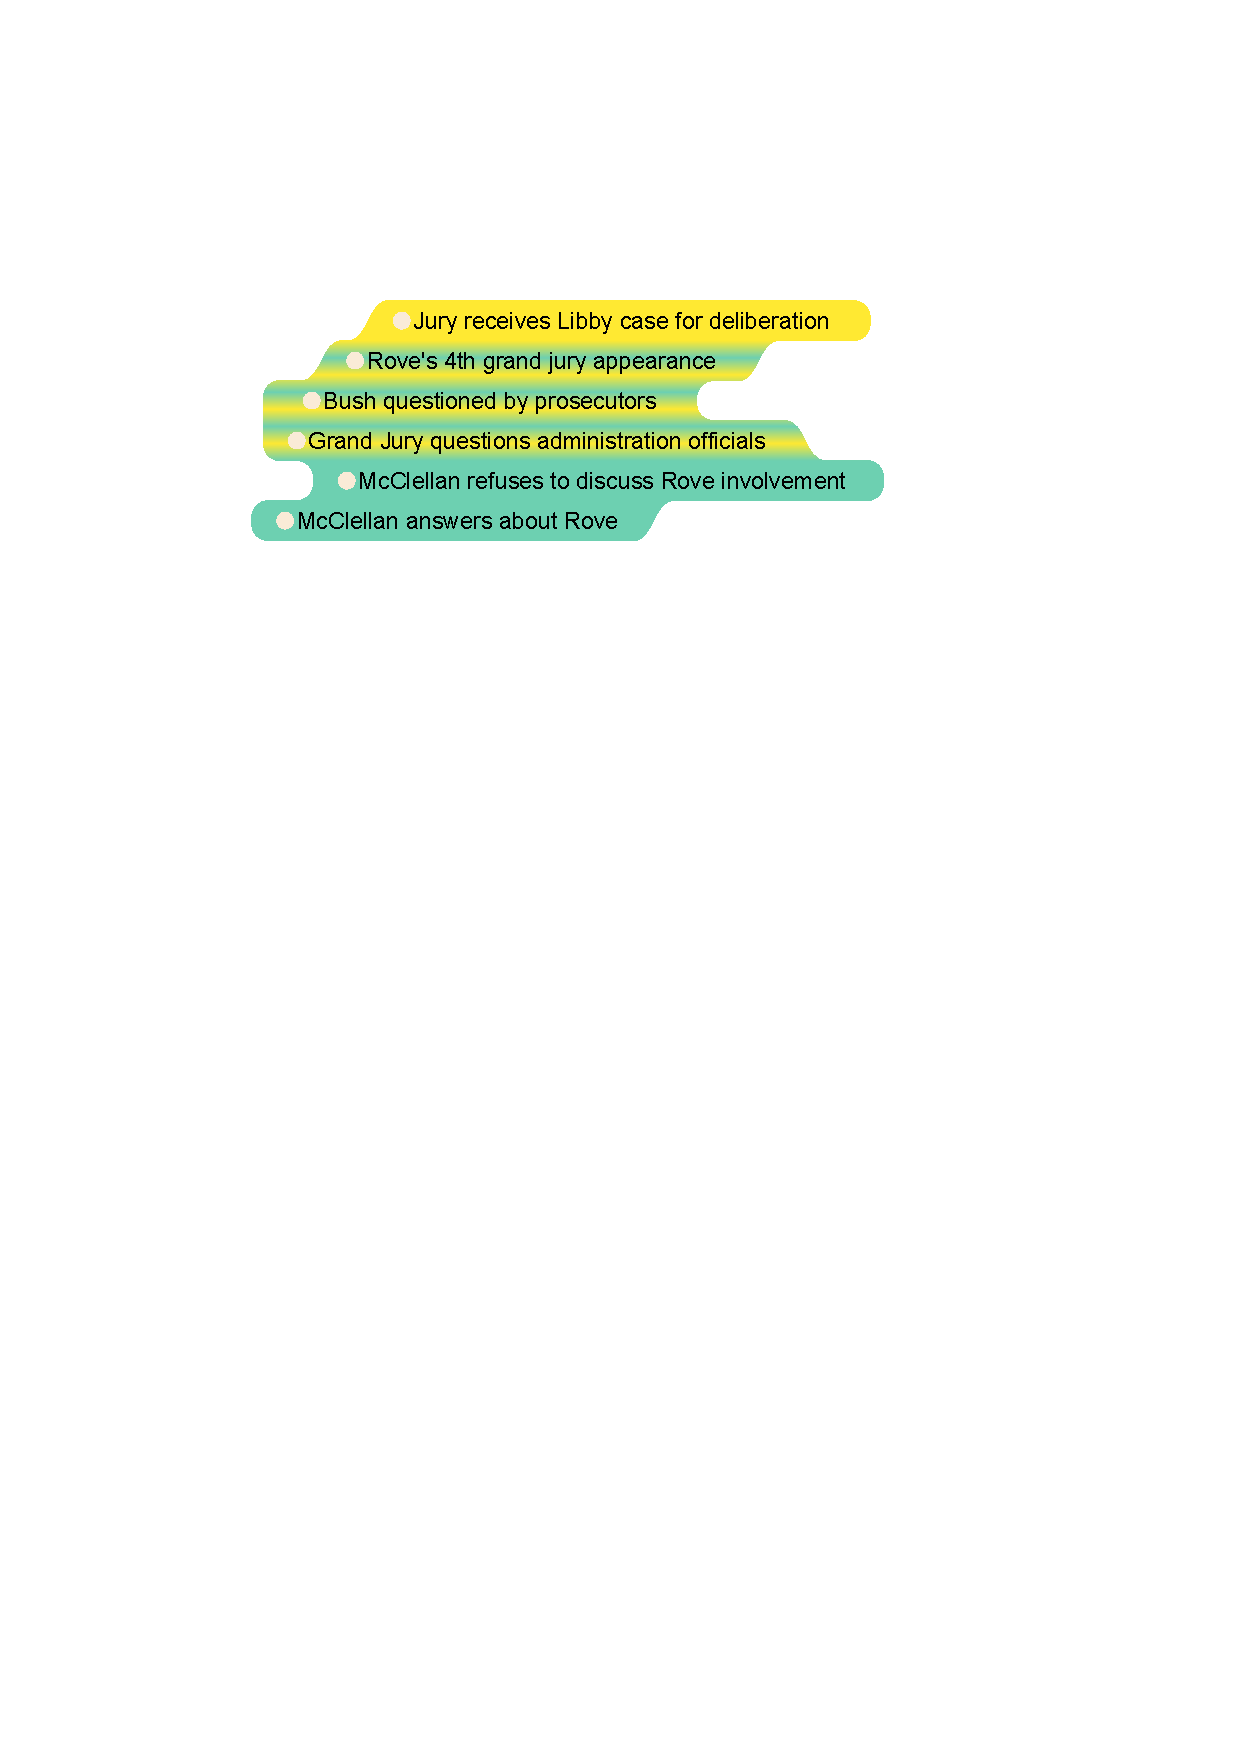
\includegraphics[width=0.48\columnwidth]{figure7b}}\label{fig:gradient2}
	\caption{Color gradient technique to encode set memberships. The gradient area shows three shared events between two sets.}
	\label{fig:gradient}
\end{figure}

\subsubsection{Multiple-set Events Visualization}
With the vertical layering of sets as discussed above, three sets cannot be placed closed to each other; therefore, it is impossible to visualize intersections among three sets or more. This is also a challenging problem with many state-of-the-art methods~\cite{Alsallakh2014}. To address this issue, similar to non-neighboring sets, we replicate events for each set they belong to so that all events in a same set stay close together providing a compact visualization and easy comparison. To provide full set memberships of events, one method is drawing edges to connect all replicates of the same event together. However, this may produce a cluttered visualization with many edge crossings. Another method is to color code the event according to its set memberships. One approach is to color the event's time icon preceding its label using either multiple circles (Figure~\ref{fig:eventmembership1}) or concentric rings (Figure~\ref{fig:eventmembership2}). The former requires more horizontal space, while the latter needs more vertical space. Another approach is to color the background of the event's label. Color gradient is used for a smooth color transition as in Figure~\ref{fig:eventmembership3}. This visual encoding is consistent with the use of color gradient to show 2-set intersections. However, a timeline with many long-label events may produce a too colorful and distracted visualization. Also, limited label height may hamper the detection of color transition. To solve these problems, color is transitioned from left to right, and only run through a first few characters of the event label. Figure~\ref{fig:citations} shows this technique in a visualization with 200 events.

\begin{figure}[ht]
	\centering
	\subcaptionbox{Each circle represents a set.}{\label{fig:eventmembership1}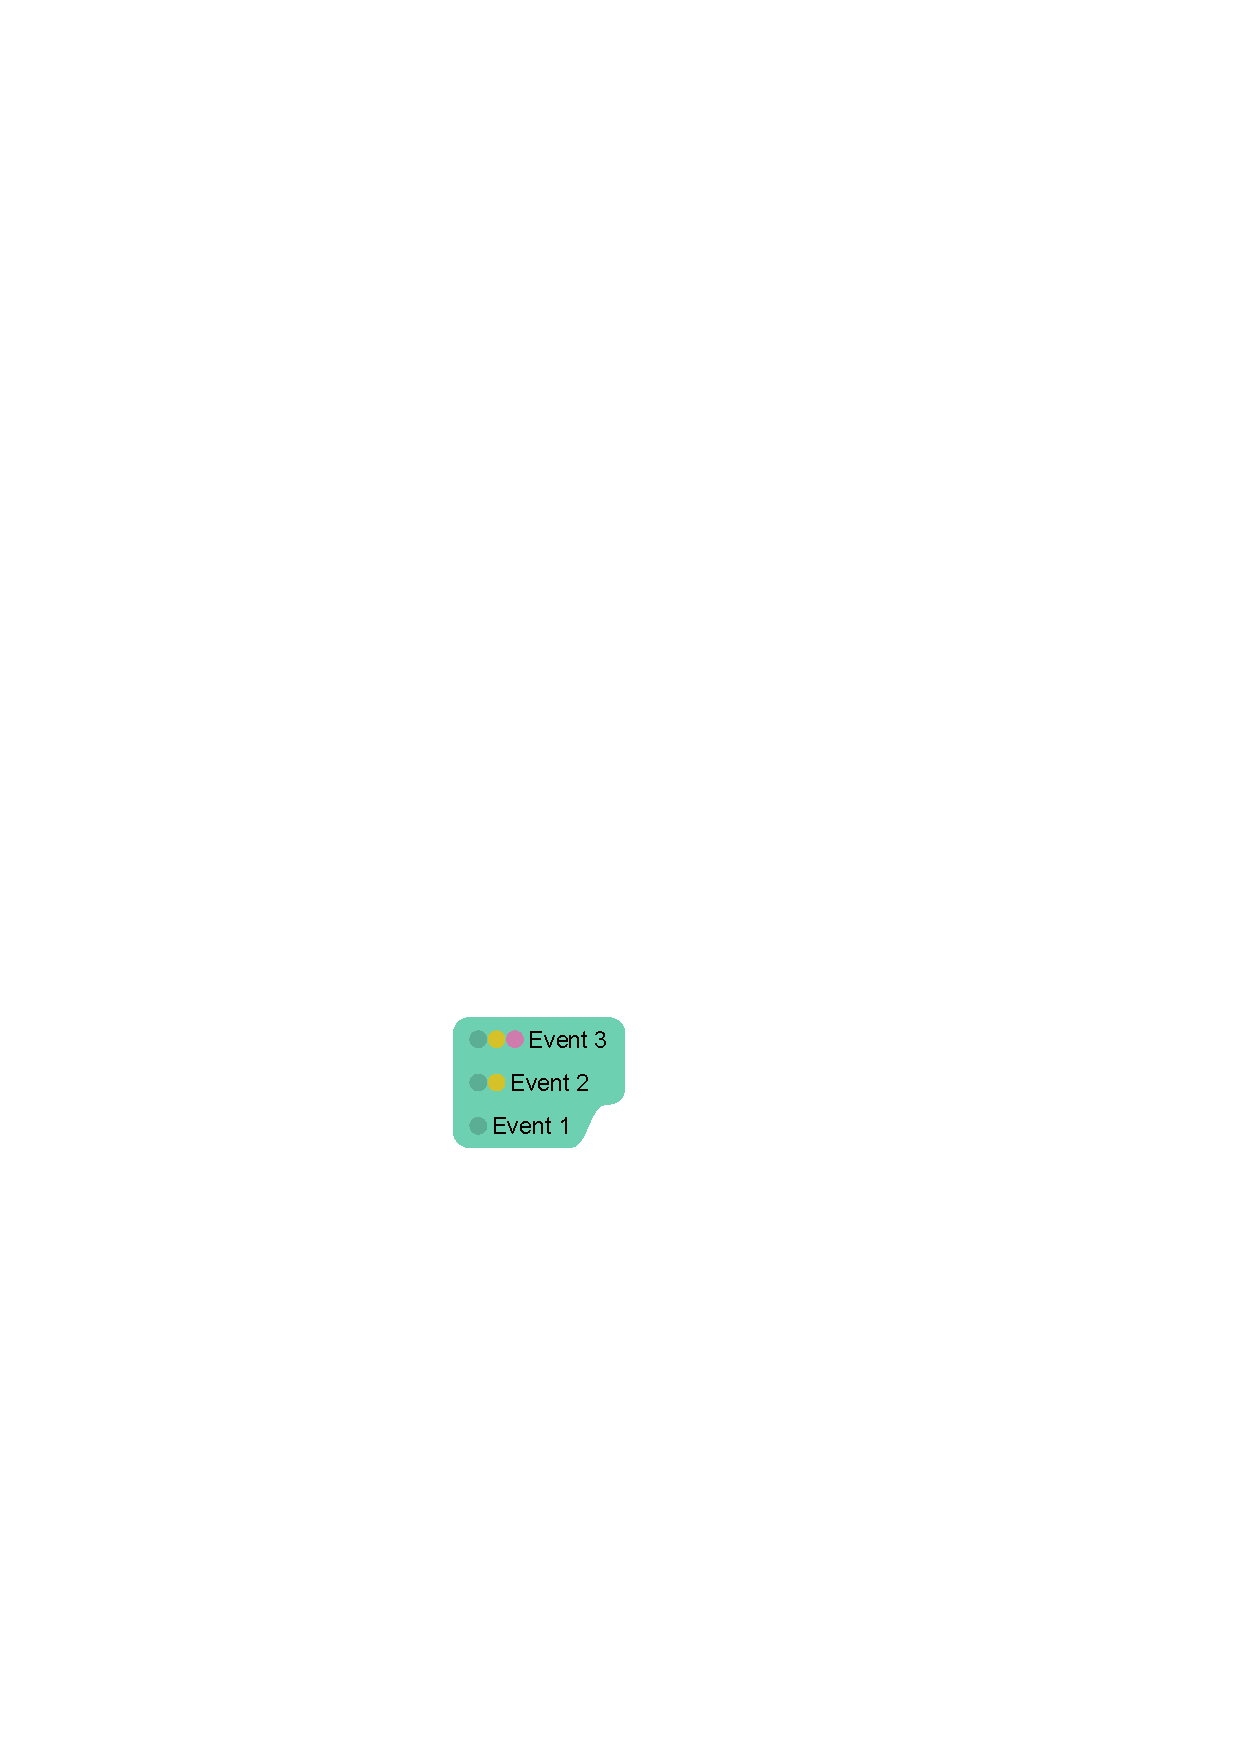
\includegraphics[width=.29\columnwidth]{figure8a}}
	\hfill
	\subcaptionbox{Each ring represents a set.}{\label{fig:eventmembership2}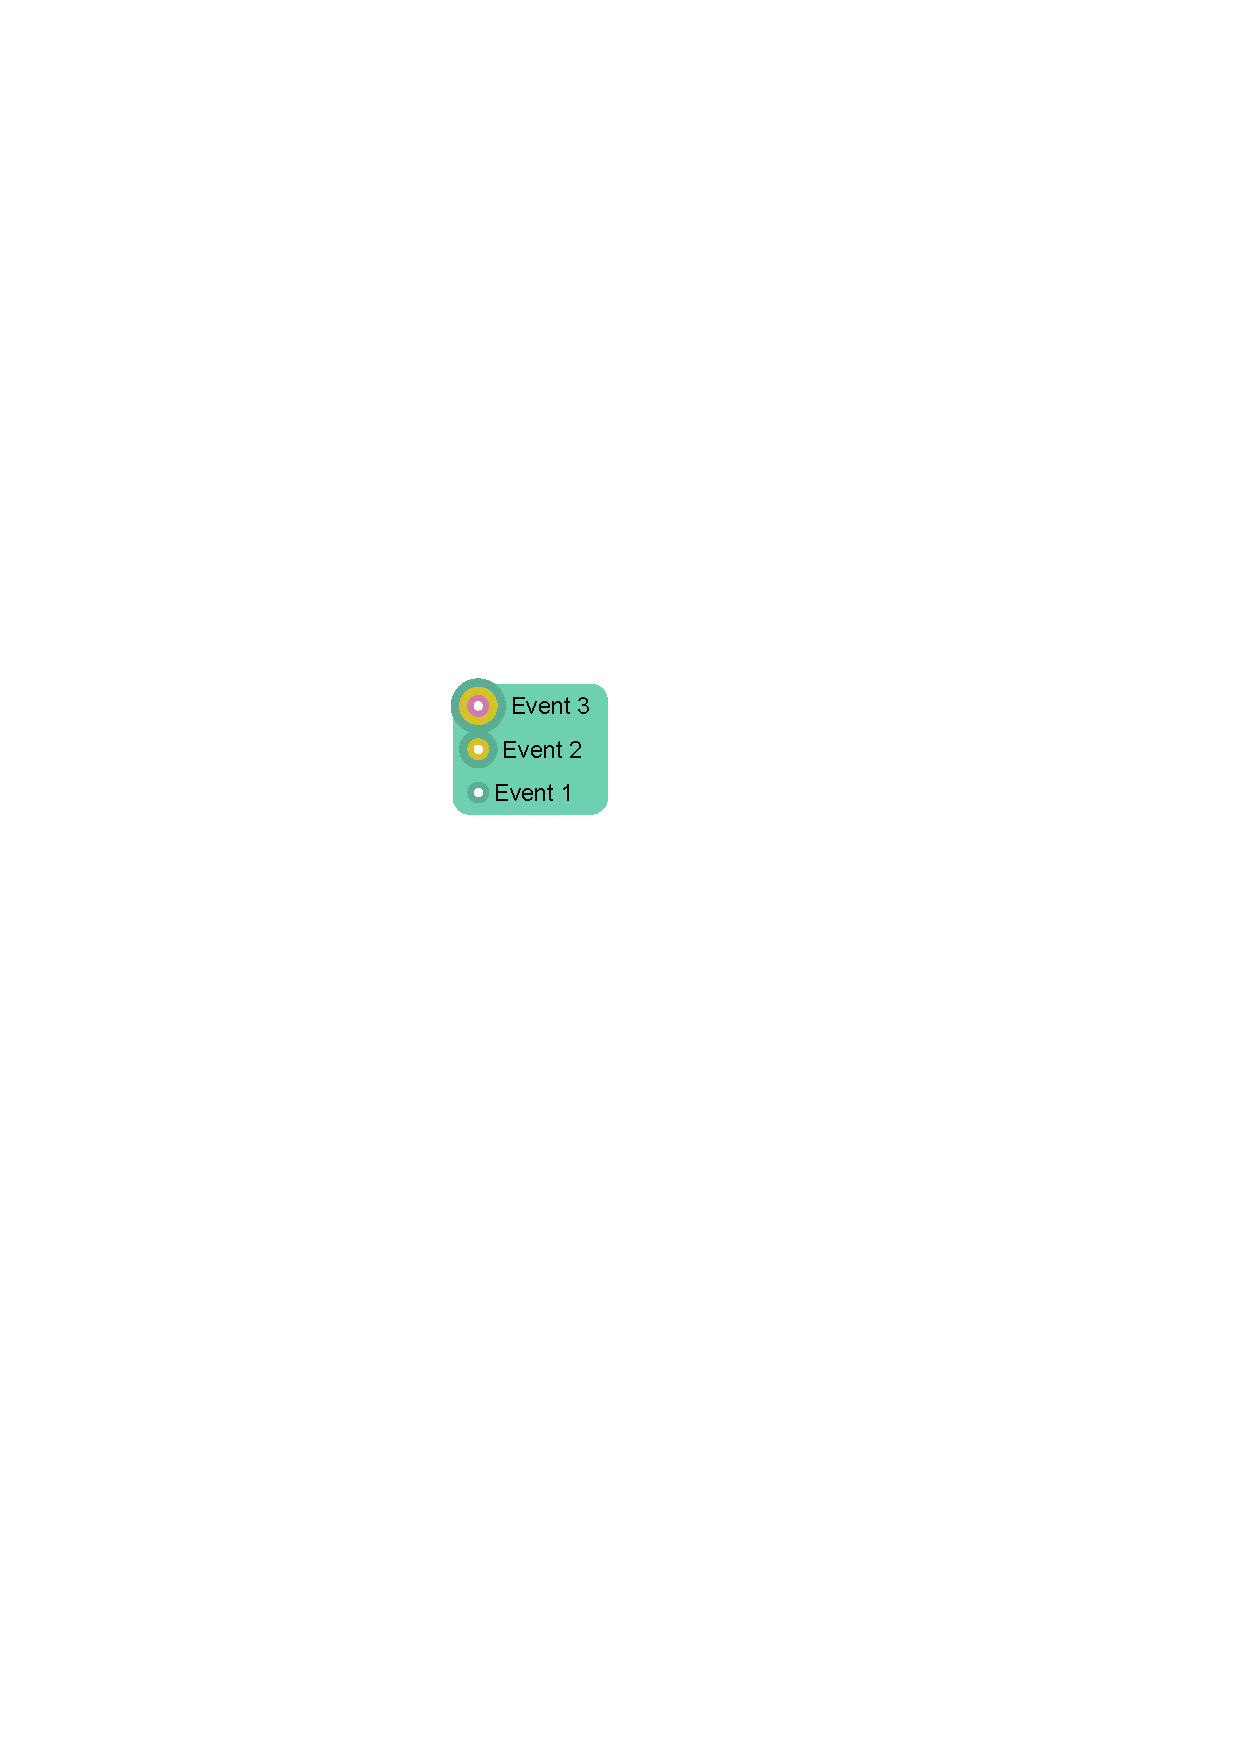
\includegraphics[width=.29\columnwidth]{figure8b}}
	\hfill
	\subcaptionbox{Each color in the gradient background represents a set.}{\label{fig:eventmembership3}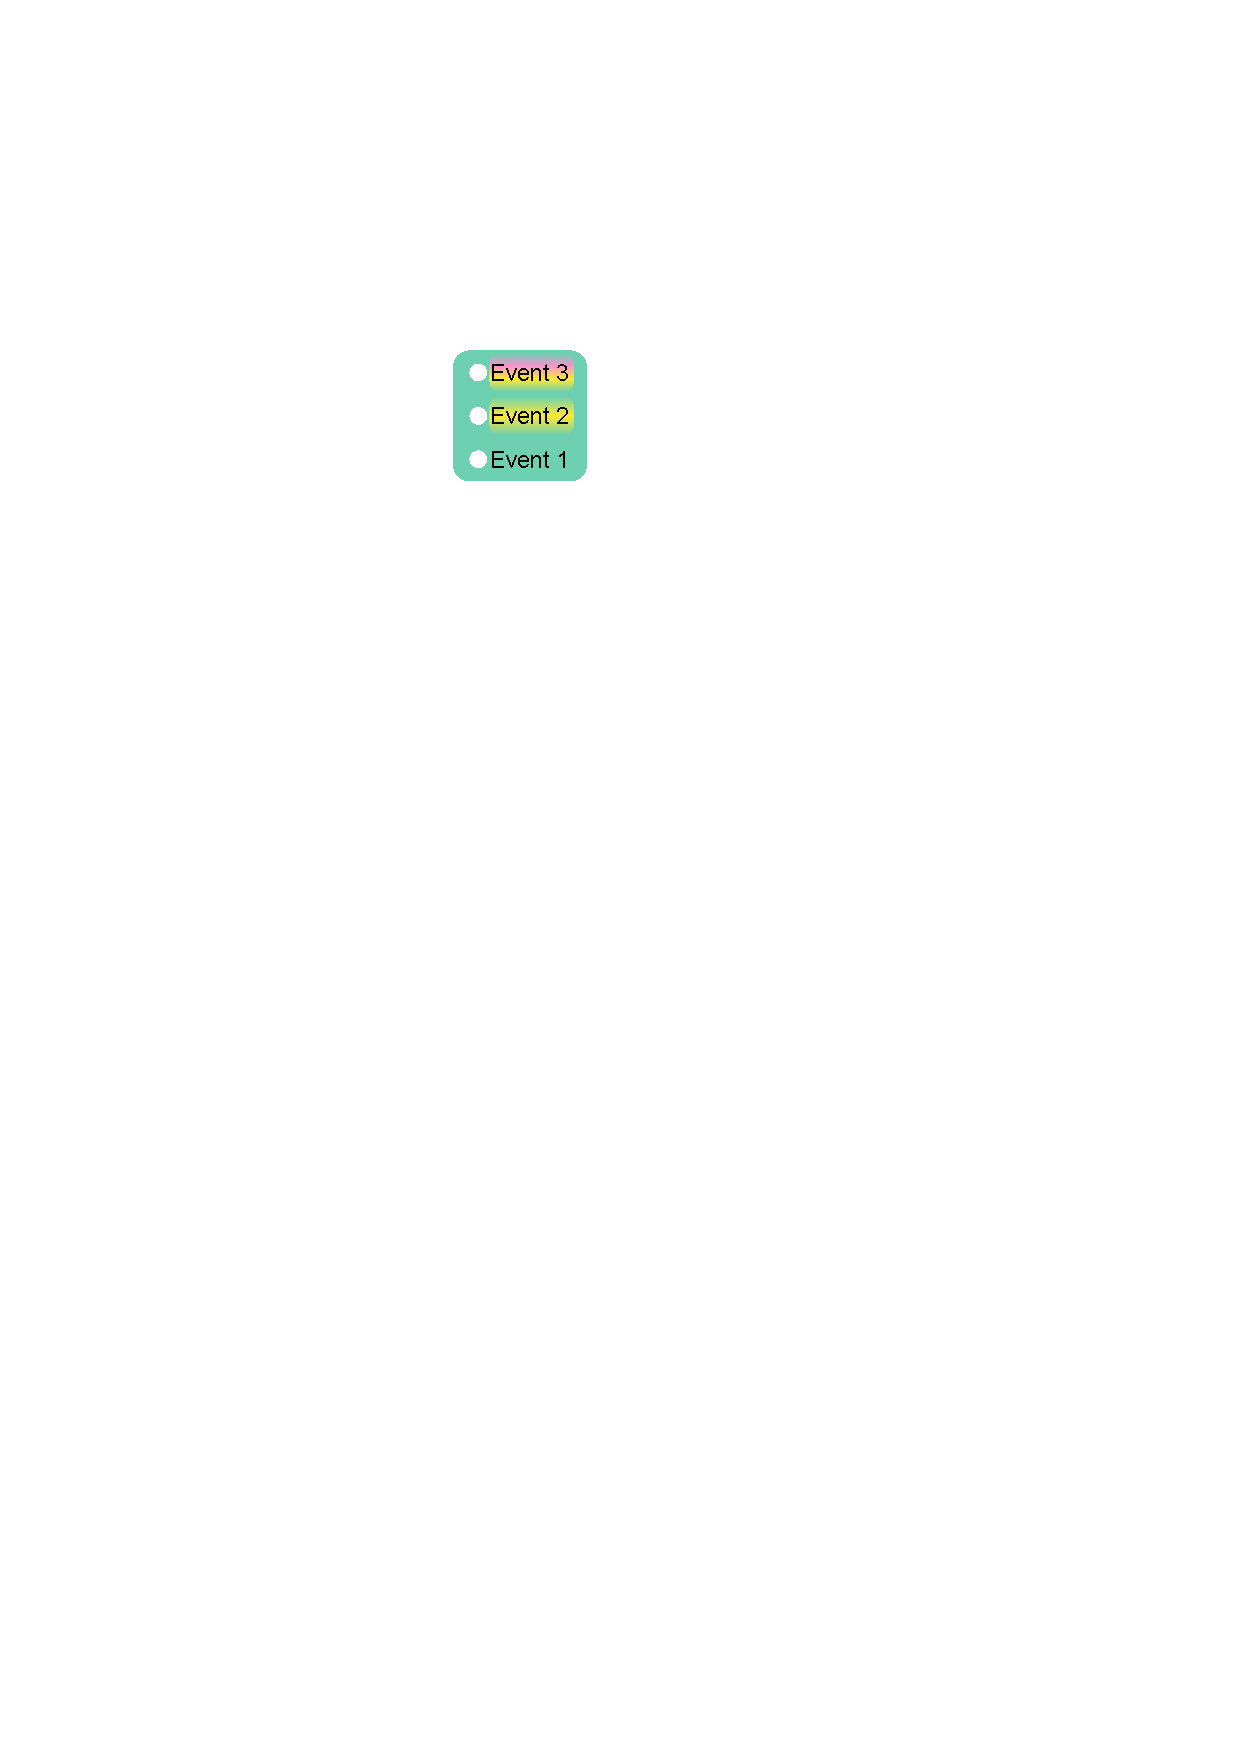
\includegraphics[width=.29\columnwidth]{figure8c}}
	\caption{Multiple-set events visualization. Event 1 is single-set. Event 2 is double-set. Event 3 is triple-set.}
	\label{fig:eventmembership}
\end{figure}

For interval events, only the label background method can work because it does not have time circles, which can be added but at the cost of extra display space. Time bars can be used to show set memberships by dividing into multiple horizontal parts, each color for one set. However, this could be mis-interpreted as an event having different set membership in each part of its timespan.

\subsection{Interaction}
\label{sub:interaction}
Interactive features are implemented to support timeline exploration. Details-on-demand provides related information without information overload. Mouse-over an event reveals its starting/ending time and complete label. When none of the multiple-set visualization techniques proposed above is used to statically display the full set memberships of an event, it is possible to use interaction to reveal that information. When an event is hovered, all of its replicates are highlighted, thus allows detecting all sets it belongs to. This method prevents adding an extra ink to the visualization; however, it requires users to discover the set information manually. 

TimeSets provides interactive set filtering and time range navigation (zooming and panning). Clicking on a set in the legend (bottom-right corner in Figure~\ref{fig:teaser}) toggles its visibility. Time range zooming is performed using the mouse-wheel and the panning is controlled by dragging. Users can also interactively modify set ordering by changing the order in the legend through drag-and-drop. A smooth animated transition is provided for all the interactions to help users maintain their mental map~\cite{Elmqvist2011}. A demonstration of these interactive features can be found in the supplemental video.